\documentclass{article}
\usepackage[utf8]{inputenc}
\usepackage{graphicx}
\usepackage{hyperref}
\usepackage{fancyhdr}
\pagestyle{fancy}

\fancyhead[LE,RO]{Jesse Both}

\hypersetup{
    colorlinks,
    citecolor=black,
    filecolor=black,
    linkcolor=black,
    urlcolor=black
}
\graphicspath{ {/graphics/} }
\title{\Huge{\textbf{CSE 321}  \\* Project 2 \\~\\ \textbf{Count-Down \\* Timer System}}}

\date{} %remove date from make title


%image

% \begin{center}
% {\includegraphics[height=10cm]{*.png}\centering}
% end{center}

\begin{document}
    \maketitle
    \vfill 
    {\Large\centering\textbf{Jesse Both  \\~\\}\par}

    {\Large\centering{Fall 2021}\par}
    {\large\centering{\today}\par}

    \newpage
    \begin{center}
        \tableofcontents
    \end{center}
\newpage
\setcounter{secnumdepth}{-1}


\section{Introduction}
The purpose of this project was to implement a count-down alarm system that utilizes bare metal methodology.
The system allows input via a 4x4 keypad and displays pertinent information to the user.  When the timer has 
run out of time, a series of alarm indicator LEDs light up.
\newline

\section{Specifications}

\begin{itemize}
    \item Time is entered in the format 'm:ss'.
    \item 'A' starts the timer.
    \item 'B' stops and turns the timer off.
    \item 'C' changes the count direction.
    \item 'D' is pressed to initiate entering a time.
    \item Bounce needs to be handled.
    \item An LED lights up after every keypress.
    \item The system runs forever.
  \end{itemize}

\section{Featrues}
The system features a 4x4 keypad where a series of interrupts are utilized to determine the key that was
pressed.  The keypad allows the user to manipulate the timer.  The user is able to input a time, start and 
stop the timer.
\newline

\noindent
An importannt feature that needed to be handled was to get rid of or reduce bounce.  In 
this system this was handled by adding a quarter second delay between each keypress.  In 
the main loop there is a thread delay of 10ms.  This quarter second key press delay was
handled by having a keypress flag and a time decrementer.  When the keypress flag was
set, the time decrementer would be a value between 1 and 25.  This value would decrement
until it is equal to 0 and the keypress flag is set to 0 to indicate that a new key can 
be pressed.  This solution is efficient because it does not lock the thread for the 
entire 250 ms.
\newline

\noindent
A 16x2 LCD is used to provide the user with a visual interface of the system.  The LCD can display prompts
for the user aswell as display the current time.
\newline

\noindent
A blue LED is used to provide the user with a visual that their keypress has been noticed by the system.
\newline

\noindent
A series of red and yellow LEDs are used to indicate when time is up.  These LEDs are programmed to light
up sequentially for an appealing visual indication.
\newline

\section{Applications}
\begin{itemize}
    \item Egg Timer
    \item Procrastination Timer
    \begin{itemize}
        \item Reduces the amount of time the user can procastinate.
      \end{itemize}
    
  \end{itemize}


\section{Block Diagram}
\begin{center}
    {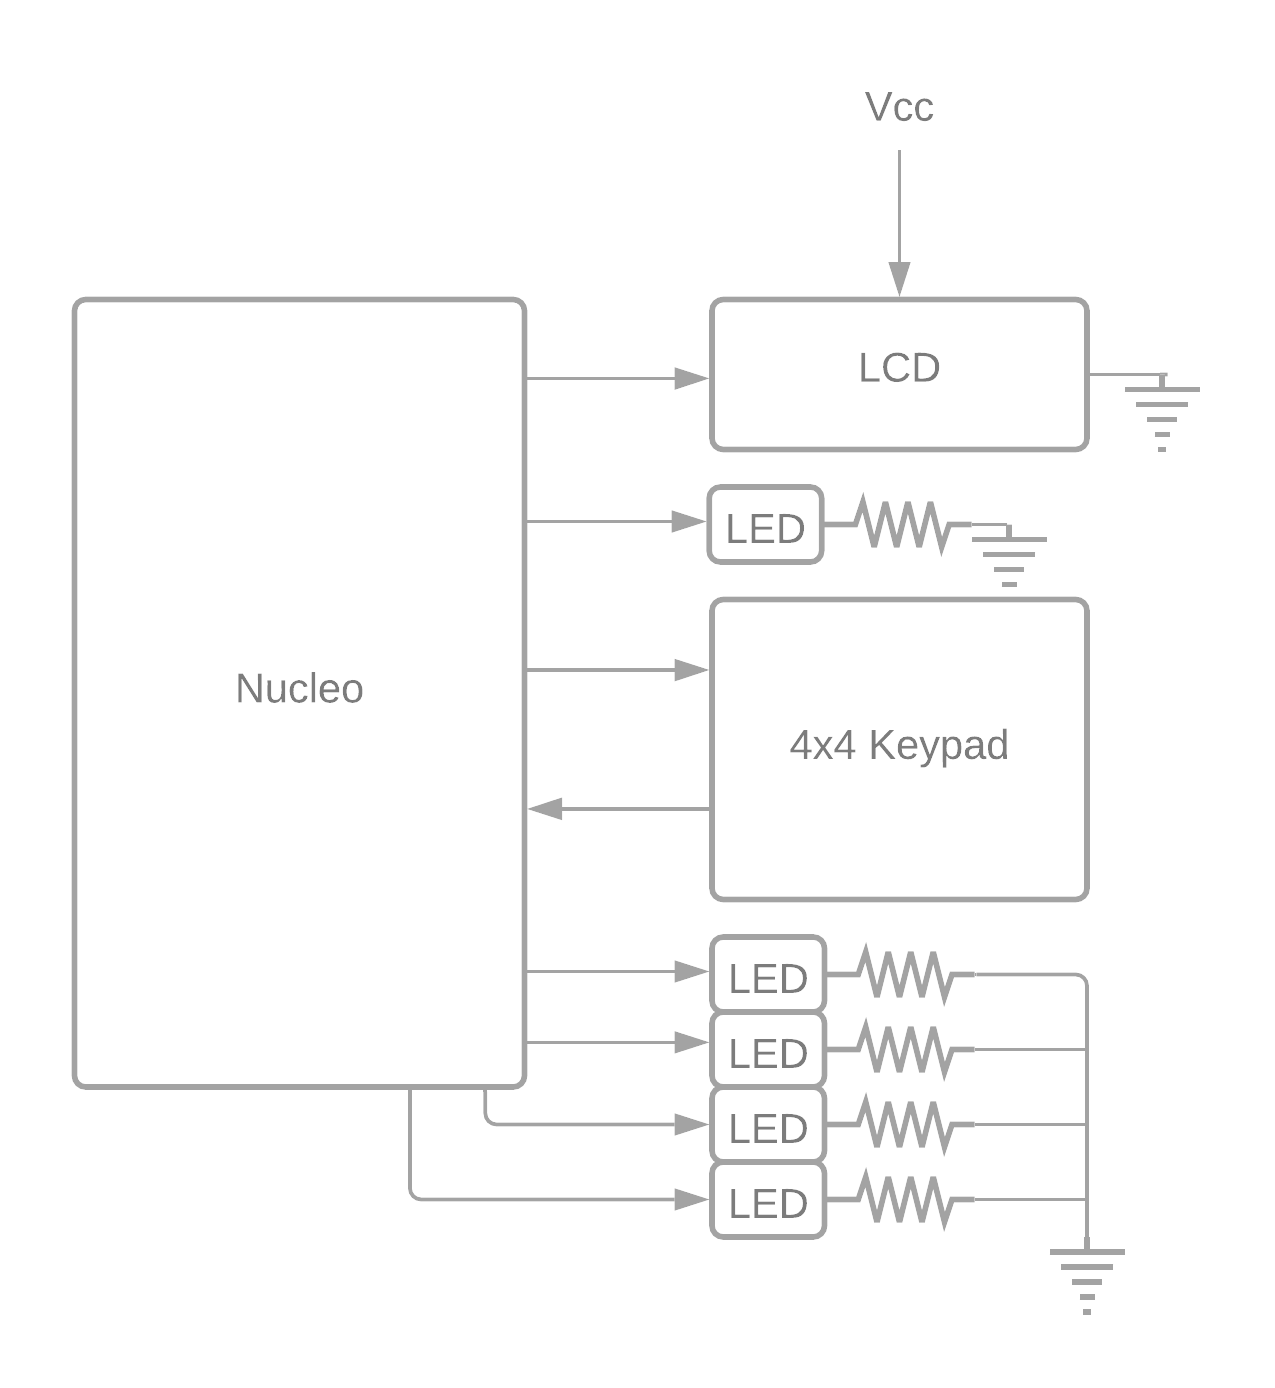
\includegraphics[height=10cm]{graphics/CSE321_project2_block_diagram.png}\centering} 
\end{center}
-
\newpage

\section{Functionality}
\begin{itemize}
    \item Press 'D' to input a time.
    \item Input a time in the format m:ss.
    \item Press 'A' to start the timer with the input time.
    \item Press 'B' to pause the timer.
    \item Press 'B' to reset or 'A' to start after pause.
    \item When the goal is reached, an LED alarm will blink.
    \item Everytime a key is pressed an indicator LED illuminates.
\end{itemize}

\subsection{Bonus Functionality}
The Bonus functionality includes an additional button input 'C'. When C is pressed
the counter direction changes and an indicator is displayed on the LCD to show
whether the alarm will be incrementing or decrementing.  'C' can be pressed when in the 
'enter time' mode.  'C' can be pressed as many times as the user want in the enter time
mode.  After each press, the timer direction is reversed.
The new functionality, including 'C' is as follows:
\begin{itemize}
    \item Press 'D' to input a time.
    \item Input a time in the format m:ss. Press 'C' to change count direction.
    \item Press 'A' to start the timer with the input time.
    \item Press 'B' to pause the timer.
    \item Press 'B' to reset or 'A' to start after pause.
    \item When the goal is reached, an LED alarm will blink.
    \item Everytime a key is pressed an indicator LED illuminates.
\end{itemize}
\newpage

\section{Diagram}
\begin{center}
    {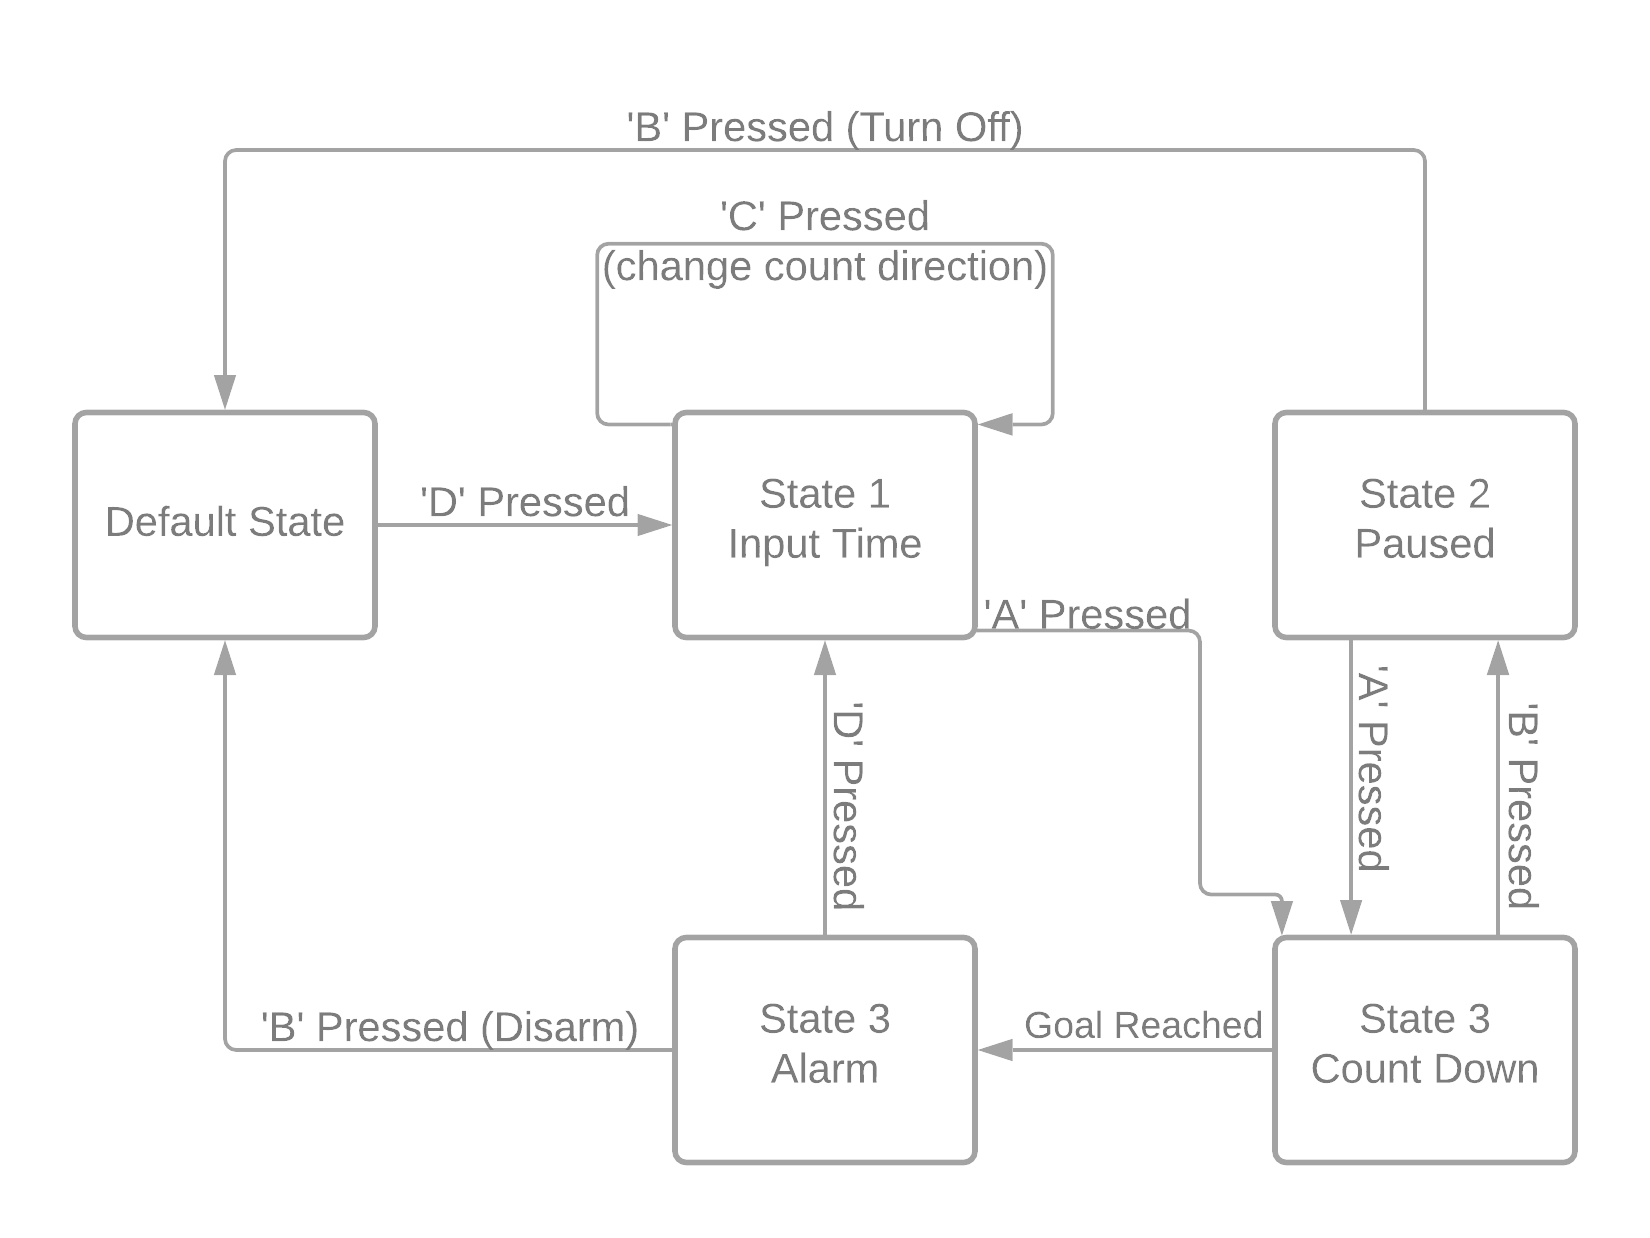
\includegraphics[height=10cm]{graphics/CSE321_project2_diagram.png}\centering} 
\end{center}

\section{BOM}
\begin{itemize}
    \item 4x4 keypad
    \item 16x2 LCD (1802)
    \item 5 LEDs
    \begin{itemize}
        \item x1 Blue
        \item x2 Yellow
        \item x2 Red 
    \end{itemize}

    \item Resistors

    \begin{itemize}
        \item x4 1k  $\Omega$ (for keypad pulldown)
        \item x5 220  $\Omega$
    \end{itemize}

  \end{itemize}

\section{Schematic}
    \begin{center}
        {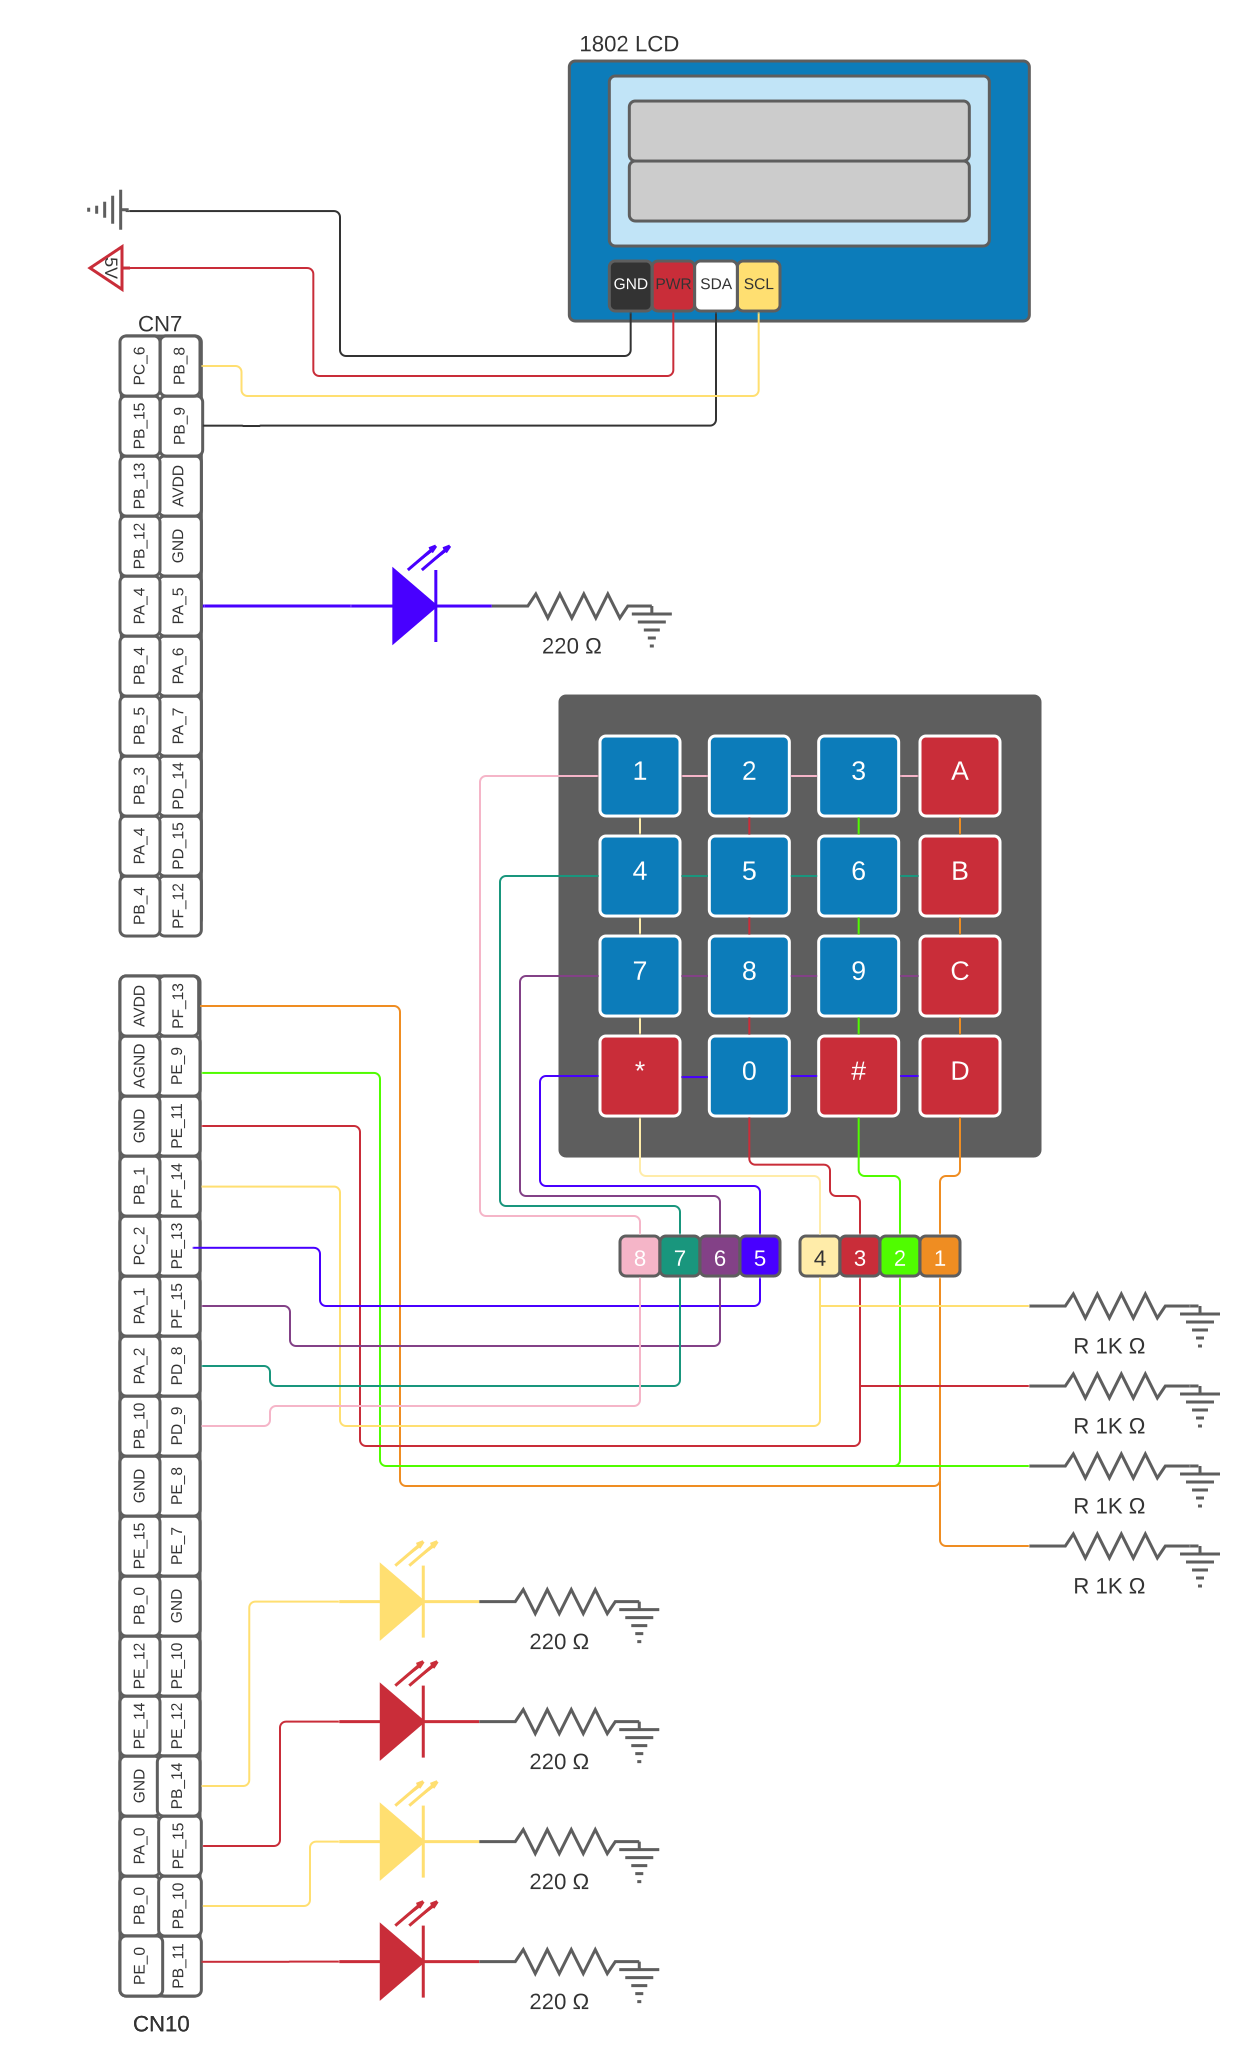
\includegraphics[height=18cm]{graphics/CSE321_project2_schematic.png}\centering} 
    \end{center}
    -
\newline

\section{Test Plan}
The test plan for this system mostly involved trial and error.  The first step to verify
the system was to make sure the count down timer functionality was working.  This was
done by hard coding a specified time and using the ticker isr to decrement the timer. 
In this process, the functionality of the timer string to minutes and second integers
was verifies as well as converting the integer minutes and seconds back into a string.  
This was necessay because after the user inputs a string in the format m:ss, this needs
to be decoded into 2 integers.  While the count down process is happending these integers
are decremented and converted to a string that is output to the LCD.
\newline

\noindent
The next step was to verify the keypad.  This was verified by using print statements 
after each key was pressed.  If the corresponding key was displayed the system is working.
One point of concern in this implementation is if the user were to manage to press a key 
between the time that the new row value is set and before the gpio pin is activated, the 
wrong key would be displayed.  The chance for this is almost 0, but it is an edge case 
that should be mentioned.
\newline

\noindent
The last step for testing was to make sure the LED functionality was correct.  Based on
the specifications of the system, an indicator LED should illuminate after each key press.
This can be tested by pressing a key and verifying that it does indeed light up.  The other
LED functionality includes and LED alarm indicator.  These LEDs should emit light when 
time is up or time has been reached.  These LEDs can be verified by setting a time
with the keypad and verifying that when the time ends that the LEDs light up.
\newline

\section{Results}
Based on the testing that took place, the system appears to work as it was designed.
The LCD displays prompts and outputs the timer in the correct format as expected.
The keypad was properly debounced and allows the user to input characters depending on
the systems state.  The LED alarm acts turns on and off as it should. The keypress indicator
LED turns on breifly when a key is pressed.
\newline

\section{Recommendations}
It is recommended to expand the timer capability.  In its current state, the timer
can only allow for input that is in the format m:ss.  In order to make the timer more
capable, it should be able to handle atleast hh:mm:ss.  Inorder to implement this
new version of the system, some adjustments would have to be made in the timer code file.
The function that need adjustments are int\_timer(), set\_press\_timer() and 
output\_press\_timer().
\newline

\end{document}